\documentclass[11pt,aspectratio=169]{beamer}\usepackage[]{graphicx}\usepackage[]{color}
% maxwidth is the original width if it is less than linewidth
% otherwise use linewidth (to make sure the graphics do not exceed the margin)
\makeatletter
\def\maxwidth{ %
  \ifdim\Gin@nat@width>\linewidth
    \linewidth
  \else
    \Gin@nat@width
  \fi
}
\makeatother

\definecolor{fgcolor}{rgb}{0.345, 0.345, 0.345}
\makeatletter
\@ifundefined{AddToHook}{}{\AddToHook{package/xcolor/after}{\definecolor{fgcolor}{rgb}{0.345, 0.345, 0.345}}}
\makeatother
\newcommand{\hlnum}[1]{\textcolor[rgb]{0.686,0.059,0.569}{#1}}%
\newcommand{\hlstr}[1]{\textcolor[rgb]{0.192,0.494,0.8}{#1}}%
\newcommand{\hlcom}[1]{\textcolor[rgb]{0.678,0.584,0.686}{\textit{#1}}}%
\newcommand{\hlopt}[1]{\textcolor[rgb]{0,0,0}{#1}}%
\newcommand{\hlstd}[1]{\textcolor[rgb]{0.345,0.345,0.345}{#1}}%
\newcommand{\hlkwa}[1]{\textcolor[rgb]{0.161,0.373,0.58}{\textbf{#1}}}%
\newcommand{\hlkwb}[1]{\textcolor[rgb]{0.69,0.353,0.396}{#1}}%
\newcommand{\hlkwc}[1]{\textcolor[rgb]{0.333,0.667,0.333}{#1}}%
\newcommand{\hlkwd}[1]{\textcolor[rgb]{0.737,0.353,0.396}{\textbf{#1}}}%
\let\hlipl\hlkwb

\usepackage{framed}
\makeatletter
\newenvironment{kframe}{%
 \def\at@end@of@kframe{}%
 \ifinner\ifhmode%
  \def\at@end@of@kframe{\end{minipage}}%
  \begin{minipage}{\columnwidth}%
 \fi\fi%
 \def\FrameCommand##1{\hskip\@totalleftmargin \hskip-\fboxsep
 \colorbox{shadecolor}{##1}\hskip-\fboxsep
     % There is no \\@totalrightmargin, so:
     \hskip-\linewidth \hskip-\@totalleftmargin \hskip\columnwidth}%
 \MakeFramed {\advance\hsize-\width
   \@totalleftmargin\z@ \linewidth\hsize
   \@setminipage}}%
 {\par\unskip\endMakeFramed%
 \at@end@of@kframe}
\makeatother

\definecolor{shadecolor}{rgb}{.97, .97, .97}
\definecolor{messagecolor}{rgb}{0, 0, 0}
\definecolor{warningcolor}{rgb}{1, 0, 1}
\definecolor{errorcolor}{rgb}{1, 0, 0}
\makeatletter
\@ifundefined{AddToHook}{}{\AddToHook{package/xcolor/after}{
\definecolor{shadecolor}{rgb}{.97, .97, .97}
\definecolor{messagecolor}{rgb}{0, 0, 0}
\definecolor{warningcolor}{rgb}{1, 0, 1}
\definecolor{errorcolor}{rgb}{1, 0, 0}
}}
\makeatother
\newenvironment{knitrout}{}{} % an empty environment to be redefined in TeX

\usepackage{alltt}

% Define the theme
\usepackage[sfmath]{kpfonts}
%\usepackage{fbb}
\usetheme[progressbar=frametitle, 
titleformat=smallcaps, 
titleformat section=smallcaps,
numbering=fraction]{metropolis}

\usepackage{tabularx}
\usepackage{booktabs}
\usepackage{amsmath}
\usepackage{amssymb}
\usepackage{stackrel}
\usepackage{geometry}
\usepackage{booktabs}
\usepackage{tikz}
\usetikzlibrary{decorations.markings}
\usetikzlibrary{shapes.geometric}
\usetikzlibrary{decorations.pathreplacing}
\IfFileExists{upquote.sty}{\usepackage{upquote}}{}
\begin{document}

\section{Basic DiD Dust-Off}


\begin{frame}
\frametitle{DiD setup}
    \centering\footnotesize
    \begin{tikzpicture}
    \node  (0) at (-1, 7) {y};
    \node  (1) at (-1, -0) {}; %Origin
    \node  (2) at (10, -0) {t};
    \draw [->] (1.center) to (2);
    \draw [->] (1.center) to (0);
    \node  (10) at (2, -0.25) {0}; % periods
    \node  (11) at (5, -0.25) {1};
    \node  (11) at (8, -0.25) {2};
    % control group
    \fill (2, 1.5) circle (2pt) node[left=2pt] {$Y_{i1}(0)\ | \ D = 0$};
    % \node  (3) at (2, 1.5) {$Y_{i1}(0)\ | \ D = 0$};
    \fill (5, 2) circle (2pt) node[above=2pt] {$Y_{i2}(0)\ | \ D = 0$};
    % \node  (4) at (5, 2) {$Y_{i2}(0)\ | \ D = 0$};
    % \fill (8, 1) circle (2pt) node[right=2pt] {$Y_{i3}(0)\ | \ D = 0$};
    % \node  (5) at (8, 1) {$Y_{i3}(0)\ | \ D = 0$};
    % \draw [thick] (8, 1) to (5, 2);
    \draw [thick] (5, 2) to (2, 1.5);
    % treatment group (observed)
    \fill (2, 4) circle (2pt) node[left=2pt] {$Y_{i1}(1)\ | \ D = 1$};
    % \node  (6) at (2, 4) {$Y_{i1}(1)\ | \ D = 1$};
    \fill (5, 6) circle (2pt) node[above=2pt] {$Y_{i2}(1)\ | \ D = 1$};
    % \node  (7) at (5, 6) {$Y_{i2}(1)\ | \ D = 1$};
    \draw [thick] (5, 6) to (2, 4);
    % treatment group (counterfactual)
    % \fill (5, 4.5) circle (2pt) node[above=2pt] {$Y_{i2}(0)\ | \ D = 1$};
    % \fill (8, 3.5) circle (2pt) node[right=2pt] {$Y_{i3}(0)\ | \ D = 1$};
    % \node  (12) at (8, 3.5) {$Y_{i3}(0)\ | \ D = 1$};
    % \draw [dash dot] (8, 3.5) to (5, 4.5);
    % \draw [dash dot] (5, 4.5) to (2, 4);
    \end{tikzpicture}
\end{frame}

\begin{frame}
\frametitle{Counterfactual outcome}
    \centering\footnotesize
    \begin{tikzpicture}
    \node  (0) at (-1, 7) {y};
    \node  (1) at (-1, -0) {}; %Origin
    \node  (2) at (10, -0) {t};
    \draw [->] (1.center) to (2);
    \draw [->] (1.center) to (0);
    \node  (10) at (2, -0.25) {0}; % periods
    \node  (11) at (5, -0.25) {1};
    % \node  (11) at (8, -0.25) {2};
    % control group
    \fill (2, 1.5) circle (2pt) node[left=2pt] {$Y_{i1}(0)\ | \ D = 0$};
    % \node  (3) at (2, 1.5) {$Y_{i1}(0)\ | \ D = 0$};
    \fill (5, 2) circle (2pt) node[above=2pt] {$Y_{i2}(0)\ | \ D = 0$};
    % \node  (4) at (5, 2) {$Y_{i2}(0)\ | \ D = 0$};
    % \fill (8, 1) circle (2pt) node[right=2pt] {$Y_{i3}(0)\ | \ D = 0$};
    % \node  (5) at (8, 1) {$Y_{i3}(0)\ | \ D = 0$};
    % \draw [thick] (8, 1) to (5, 2);
    \draw [thick] (5, 2) to (2, 1.5);
    % treatment group (observed)
    \fill (2, 4) circle (2pt) node[left=2pt] {$Y_{i1}(1)\ | \ D = 1$};
    % \node  (6) at (2, 4) {$Y_{i1}(1)\ | \ D = 1$};
    \fill (5, 6) circle (2pt) node[above=2pt] {$Y_{i2}(1)\ | \ D = 1$};
    % \node  (7) at (5, 6) {$Y_{i2}(1)\ | \ D = 1$};
    % \fill (8, 5.5) circle (2pt) node[right=2pt] {$Y_{i3}(1)\ | \ D = 1$};
    % \node  (8) at (8, 5.5) {$Y_{i3}(1)\ | \ D = 1$};
    \draw [thick] (5, 6) to (2, 4);
    % \draw [thick] (8, 5.5) to (5, 6);
    % treatment group (counterfactual)
    \fill (5, 4.5) circle (2pt) node[above=2pt] {$Y_{i2}(0)\ | \ D = 1$};
    % \fill (8, 3.5) circle (2pt) node[right=2pt] {$Y_{i3}(0)\ | \ D = 1$};
    % \node  (12) at (8, 3.5) {$Y_{i3}(0)\ | \ D = 1$};
    % \draw [dash dot] (8, 3.5) to (5, 4.5);
    \draw [dash dot] (5, 4.5) to (2, 4);
    \end{tikzpicture}
\end{frame}

\begin{frame}
\frametitle{Counterfactual outcome}
    \centering\footnotesize
    \begin{tikzpicture}
    \node  (0) at (-1, 7) {y};
    \node  (1) at (-1, -0) {}; %Origin
    \node  (2) at (10, -0) {t};
    \draw [->] (1.center) to (2);
    \draw [->] (1.center) to (0);
    \node  (10) at (2, -0.25) {0}; % periods
    \node  (11) at (5, -0.25) {1};
    % \node  (11) at (8, -0.25) {2};
    % control group
    \fill (2, 1.5) circle (2pt) node[left=2pt] {$Y_{i1}(0)\ | \ D = 0$};
    % \node  (3) at (2, 1.5) {$Y_{i1}(0)\ | \ D = 0$};
    \fill (5, 2) circle (2pt) node[above=2pt] {$Y_{i2}(0)\ | \ D = 0$};
    % \node  (4) at (5, 2) {$Y_{i2}(0)\ | \ D = 0$};
    % \fill (8, 1) circle (2pt) node[right=2pt] {$Y_{i3}(0)\ | \ D = 0$};
    % \node  (5) at (8, 1) {$Y_{i3}(0)\ | \ D = 0$};
    % \draw [thick] (8, 1) to (5, 2);
    \draw [thick] (5, 2) to (2, 1.5);
    % treatment group (observed)
    \fill (2, 4) circle (2pt) node[left=2pt] {$Y_{i1}(1)\ | \ D = 1$};
    % \node  (6) at (2, 4) {$Y_{i1}(1)\ | \ D = 1$};
    \fill (5, 6) circle (2pt) node[above=2pt] {$Y_{i2}(1)\ | \ D = 1$};
    % \node  (7) at (5, 6) {$Y_{i2}(1)\ | \ D = 1$};
    % \fill (8, 5.5) circle (2pt) node[right=2pt] {$Y_{i3}(1)\ | \ D = 1$};
    % \node  (8) at (8, 5.5) {$Y_{i3}(1)\ | \ D = 1$};
    \draw [thick] (5, 6) to (2, 4);
    % \draw [thick] (8, 5.5) to (5, 6);
    % treatment group (counterfactual)
    \fill (5, 4.5) circle (2pt) node[above=2pt] {$Y_{i2}(0)\ | \ D = 1$};
    % \fill (8, 3.5) circle (2pt) node[right=2pt] {$Y_{i3}(0)\ | \ D = 1$};
    % \node  (12) at (8, 3.5) {$Y_{i3}(0)\ | \ D = 1$};
    % \draw [dash dot] (8, 3.5) to (5, 4.5);
    \draw [dash dot] (5, 4.5) to (2, 4);
    % legend
    \node  (13) at (9.5, 4.5) {%
    $\begin{aligned}
    \tau = & E\left[ Y_{i2}(1) - Y_{i1}(1) \ | \ D = 1\right] -\\ 
           & E\left[ Y_{i2}(0) - Y_{i1}(0) \ | \ D = 0\right]
    \end{aligned}$
    };
    \end{tikzpicture}
\end{frame}

\begin{frame}
\frametitle{Three-period DiD}
    \centering\footnotesize
    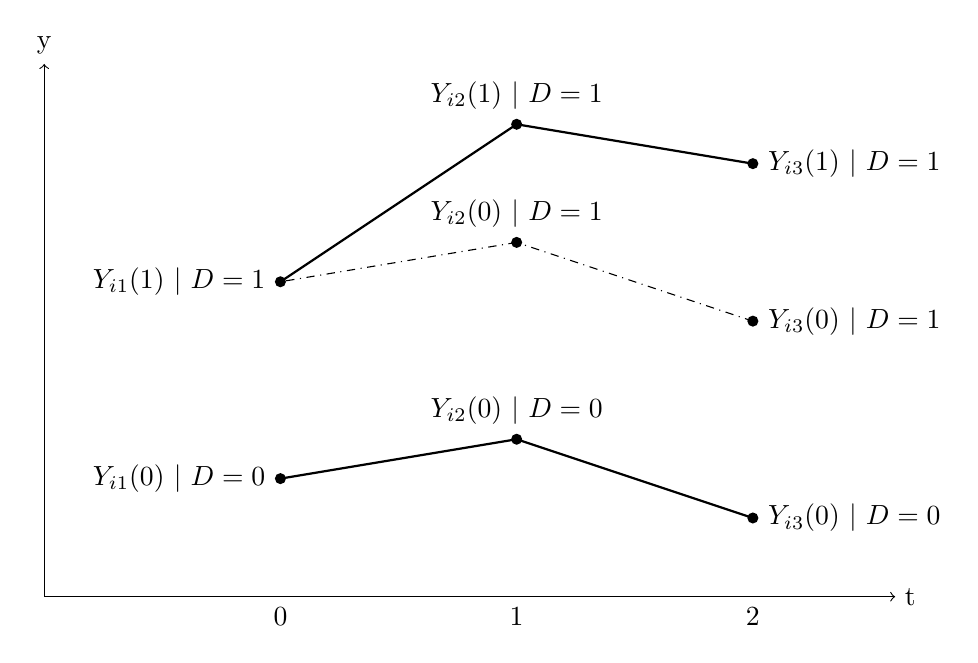
\begin{tikzpicture}
    \node  (0) at (-1, 7) {y};
    \node  (1) at (-1, -0) {}; %Origin
    \node  (2) at (10, -0) {t};
    \draw [->] (1.center) to (2);
    \draw [->] (1.center) to (0);
    \node  (10) at (2, -0.25) {0}; % periods
    \node  (11) at (5, -0.25) {1};
    \node  (11) at (8, -0.25) {2};
    % control group
    \fill (2, 1.5) circle (2pt) node[left=2pt] {$Y_{i1}(0)\ | \ D = 0$};
    % \node  (3) at (2, 1.5) {$Y_{i1}(0)\ | \ D = 0$};
    \fill (5, 2) circle (2pt) node[above=2pt] {$Y_{i2}(0)\ | \ D = 0$};
    % \node  (4) at (5, 2) {$Y_{i2}(0)\ | \ D = 0$};
    \fill (8, 1) circle (2pt) node[right=2pt] {$Y_{i3}(0)\ | \ D = 0$};
    % \node  (5) at (8, 1) {$Y_{i3}(0)\ | \ D = 0$};
    \draw [thick] (8, 1) to (5, 2);
    \draw [thick] (5, 2) to (2, 1.5);
    % treatment group (observed)
    \fill (2, 4) circle (2pt) node[left=2pt] {$Y_{i1}(1)\ | \ D = 1$};
    % \node  (6) at (2, 4) {$Y_{i1}(1)\ | \ D = 1$};
    \fill (5, 6) circle (2pt) node[above=2pt] {$Y_{i2}(1)\ | \ D = 1$};
    % \node  (7) at (5, 6) {$Y_{i2}(1)\ | \ D = 1$};
    \fill (8, 5.5) circle (2pt) node[right=2pt] {$Y_{i3}(1)\ | \ D = 1$};
    % \node  (8) at (8, 5.5) {$Y_{i3}(1)\ | \ D = 1$};
    \draw [thick] (5, 6) to (2, 4);
    \draw [thick] (8, 5.5) to (5, 6);
    % treatment group (counterfactual)
    \fill (5, 4.5) circle (2pt) node[above=2pt] {$Y_{i2}(0)\ | \ D = 1$};
    \fill (8, 3.5) circle (2pt) node[right=2pt] {$Y_{i3}(0)\ | \ D = 1$};
    % \node  (12) at (8, 3.5) {$Y_{i3}(0)\ | \ D = 1$};
    \draw [dash dot] (8, 3.5) to (5, 4.5);
    \draw [dash dot] (5, 4.5) to (2, 4);
    % other
    % \node  (15) at (3.55, 2.35) {}; %additional
    % \node  (16) at (3.55, 1.3) {$\gamma$};
    % \node  (17) at (1.5, 1.5) {$\beta_1$};
    % \node  (18) at (-0.2, 2) {$\alpha$};%
    % 
    % \draw [thick] (5.center) to (6.center);
    % \draw [thick] (4.center) to (3.center);
    % \draw [dash dot] (9.center) to (3.center);
    % \draw [thick] (3.center) to (8.center); %dashed
    % \draw [thick] (6.center) to (7.center);
    % \draw [decorate,decoration={brace,raise=4pt},yshift=0pt] (8) to (9.center); %lower bracket
    % \draw [decorate,decoration={brace,raise=4pt},yshift=0pt] (6) to (12.center); %upper bracket
    % \draw [decorate,decoration={brace,raise=4pt},yshift=0pt] (3) to (6); %upper bracket
    \end{tikzpicture}
\end{frame}




\end{document}
